\documentclass[11pt]{article}
\usepackage{amsmath}
\usepackage[margin=0.68in]{geometry}
\usepackage{booktabs}
\usepackage{enumitem}
\usepackage{fancyhdr}
\usepackage{graphicx}
\usepackage[table]{xcolor}
\usepackage[hidelinks]{hyperref}
\usepackage{listings}
\usepackage{microtype}
\usepackage{tabularx}
\usepackage{titlesec}
\graphicspath{{docs/lessons/assets/}{../assets/}}
\definecolor{Ink}{gray}{0}
\definecolor{CodeGray}{gray}{0.96}
\hypersetup{hidelinks,pdftitle={ADK Lesson 036: Magnetic Passage Logger},
 pdfauthor={Kevin Shanahan},
 pdfsubject={Durable two-slot passage records, recovery, retries, and evidence presentation},
 pdflang={en-US}}
\pagestyle{fancy}\fancyhf{}
\lhead{\textsc{ADK Lesson 036}}\rhead{Magnetic Passage Logger}
\cfoot{\thepage}\setlength{\headheight}{14pt}
\setlength{\parindent}{0pt}\setlength{\parskip}{5pt}
\setlist{nosep,leftmargin=1.45em}
\titleformat{\section}{\Large\bfseries\color{Ink}}{\thesection}{0.5em}{}
\lstdefinestyle{adkcpp}{language=C++,backgroundcolor=\color{CodeGray},
 basicstyle=\ttfamily\small,keywordstyle=\color{Ink}\bfseries,
 commentstyle=\color{Ink},columns=fullflexible,keepspaces=true,
 showstringspaces=false,frame=single,rulecolor=\color{Ink},
 breaklines=true,tabsize=4}
\newcommand{\lessonbox}[1]{%
 \begin{center}\fcolorbox{Ink}{white}{\parbox{0.92\linewidth}{#1}}\end{center}}

\begin{document}
\begin{center}
 {\Huge\bfseries Magnetic Passage Logger}\\[4pt]
 {\Large Commit accepted evidence before presenting a count}\\[8pt]
 \textit{Freeze, timestamp, persist, recover, then display}
\end{center}
\begin{tabularx}{\linewidth}{@{}>{\bfseries}l X >{\bfseries}l X@{}}
Lesson & 036 --- project & Time & 180--240 minutes\\
Prerequisites & Lessons 010, 022, 034, and 035 & Board & Mega fixture\\
Evidence & three LEDs, one digit, two host slots & Status & host verified; bench open\\
Energy class & E0 core and persistence fixtures; provisional E1 indicators\\
\end{tabularx}

\lessonbox{\textbf{Scope gate.} The project consumes accepted software records.
It does not resample sensors, decode an encoder, implement a filesystem, move a
gate, identify a person, or actuate a load. Its RTC, byte storage, and passage
inputs are deterministic host fixtures. Physical RTC, removable media,
magnetic specimens, and persistence acceptance remain open.}

\section{Mission and durable evidence}
The project preserves:
\[
\text{accepted passage}\rightarrow\text{frozen clock and label}
\rightarrow\text{durable commit}\rightarrow\text{presented count}.
\]
A label \texttt{None/A/B/C} is local metadata, never identity,
authentication, access authority, or a safety decision. A degraded
\texttt{ClockReading} remains degraded; the logger never calls it a valid
timestamp.

\section{Build one commit in visible stages}
\begin{center}
% ADK visual: pencil
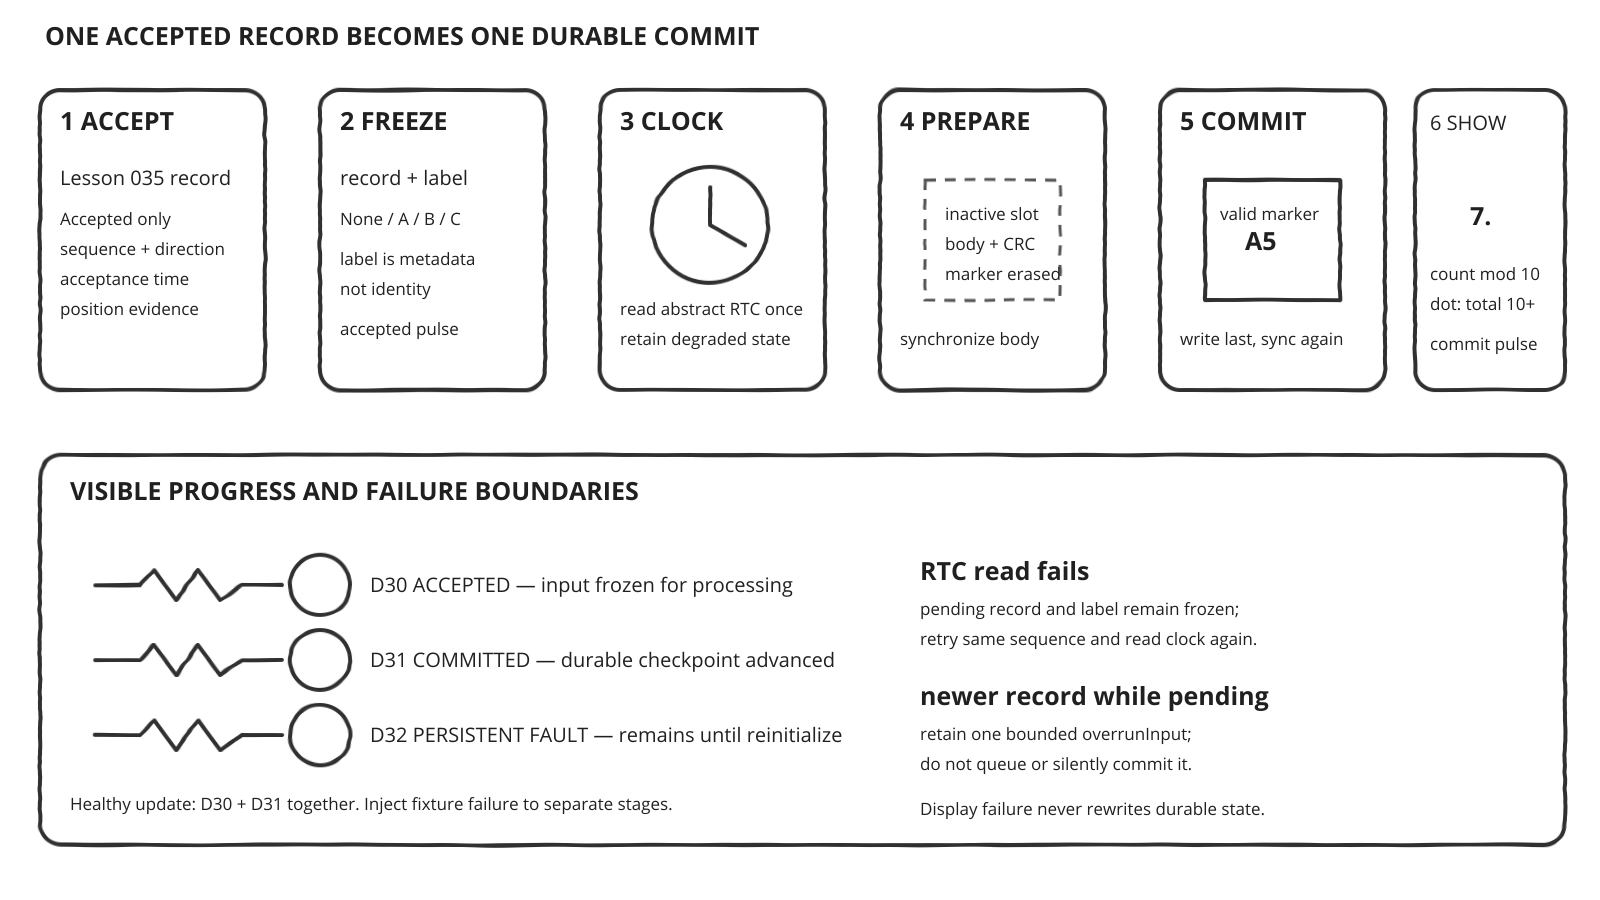
\includegraphics[width=0.98\linewidth]{036-commit-journey-pencil.png}

\small\textit{Alternative text: six pencil stages freeze one accepted record
and local label, read the abstract clock, prepare and synchronize an inactive
slot, write the valid marker last, then present the committed count; side
paths show RTC retry, bounded overrun, and three evidence LEDs.}
\end{center}

The dependent progression is visible. D30 means an accepted record was frozen;
D31 means the ledger advanced its durable checkpoint. On an immediate
successful update both pulses are true in the same snapshot. To observe the
stages separately, deliberately fail the RTC or ledger in the deterministic
fixture: D30 appears without D31, then a same-sequence retry can produce D31.
D32 holds a persistent fault until successful shutdown and reinitialization.
The one-digit display changes only after commit: it shows
\(\texttt{committedCount}\bmod10\), with decimal point meaning ten or more.

\begin{tabularx}{\linewidth}{@{}l l X@{}}
\toprule
Evidence path & Fixture role & Meaning\\
\midrule
D30 through 1 k\(\Omega\) & accepted pulse & record accepted for processing\\
D31 through 1 k\(\Omega\) & committed pulse & durable checkpoint advanced\\
D32 through 1 k\(\Omega\) & persistent fault & retry/recovery/presentation fault\\
D22/D23/D24 & 74HC595 data/clock/latch & committed count presentation only\\
D28 & label button & previews \texttt{-/A/b/C}, then restores durable count\\
\bottomrule
\end{tabularx}

These provisional roles are not a sensor or storage schematic. The known
indicator/segment bound is 55 mA: three direct LEDs at no more than 5 mA each
plus Lesson 010's 40 mA segment total. It excludes the Mega baseline, shift
register package current, sensor modules, and pulls.

\section{Logger contract}
\texttt{MagneticPassageLogger} borrows an abstract \texttt{Rtc} and one
\texttt{PassageLedger}. It presents the durable count through the narrow
\texttt{PassageCountDisplay} boundary. A lesson-local seven-segment adapter
binds the inert display to that boundary. Initialization
validates configuration, initializes ledger then RTC then display, recovers a
checkpoint, and rolls back in reverse order. Shutdown is idempotent.

\texttt{LoggedPassage} retains accepted sequence, resulting committed count,
acceptance time, direction, frozen label, copied position evidence, complete
clock reading, and explicit sequence-gap evidence.

\begin{tabularx}{\linewidth}{@{}l X@{}}
\toprule
Snapshot field & Meaning\\
\midrule
\texttt{selectedLabel} & metadata selected for the next new sequence\\
\texttt{committedCount/Sequence} & recovered or newly durable authority\\
\texttt{pending}, \texttt{pendingInput} & frozen input awaiting clock or ledger\\
\texttt{overrun}, \texttt{overrunInput} & one bounded newer input, not queued\\
\texttt{hasFrozenEntry}, \texttt{frozenEntry} & immutable bytes after RTC success\\
\texttt{acceptedPulse/committedPulse} & one-call evidence intents\\
\texttt{persistentFault} & latched fault intent\\
\texttt{recovery}, \texttt{presentationStatus}, \texttt{status} & explicit outcomes\\
\bottomrule
\end{tabularx}

Only an \texttt{Accepted} Lesson 035 record is consumable. An older sequence is
rejected. An equal sequence is idempotent only when direction, acceptance time,
and position agree with recovered durable evidence; disagreement is an
invariant fault. A forward gap may commit, but \texttt{sequenceGap} records it.

\section{Clock, retry, and overrun}
For a new sequence, the logger freezes record and current label, then attempts
one RTC read per update. A failed read emits accepted evidence, performs no
ledger or display work, and leaves the input pending. Retrying the same
sequence reads the RTC again. The first successful clock reading becomes part
of an immutable frozen entry and is never reread during ledger retries.

A failed ledger commit changes no committed count, sequence, display, or
generation. Retrying the same sequence uses byte-identical entry data. While
pending, one newer record becomes bounded \texttt{overrunInput}; later arrivals
replace that evidence. It is neither queued nor silently committed.

Presentation happens after durability. Display failure cannot change committed
state or trigger a ledger retry; it records presentation status and latches the
fault witness. A simultaneous label-button edge applies only to the next
record because the pending label was already frozen.

The canonical sketch makes label selection board-visible without confusing it
with durable authority. A D28 press briefly previews \texttt{-}, \texttt{A},
\texttt{b}, or \texttt{C} for \texttt{None/A/B/C}; after one second it restores
the committed count and decimal-point convention. The sketch preserves the
pre-cycle D30/D31 pulse intents, checks \texttt{cycleLabel()}, refreshes the
post-cycle snapshot, and never treats the temporary glyph as a committed
count.

\section{Two-slot recovery}
\begin{center}
% ADK visual: pencil
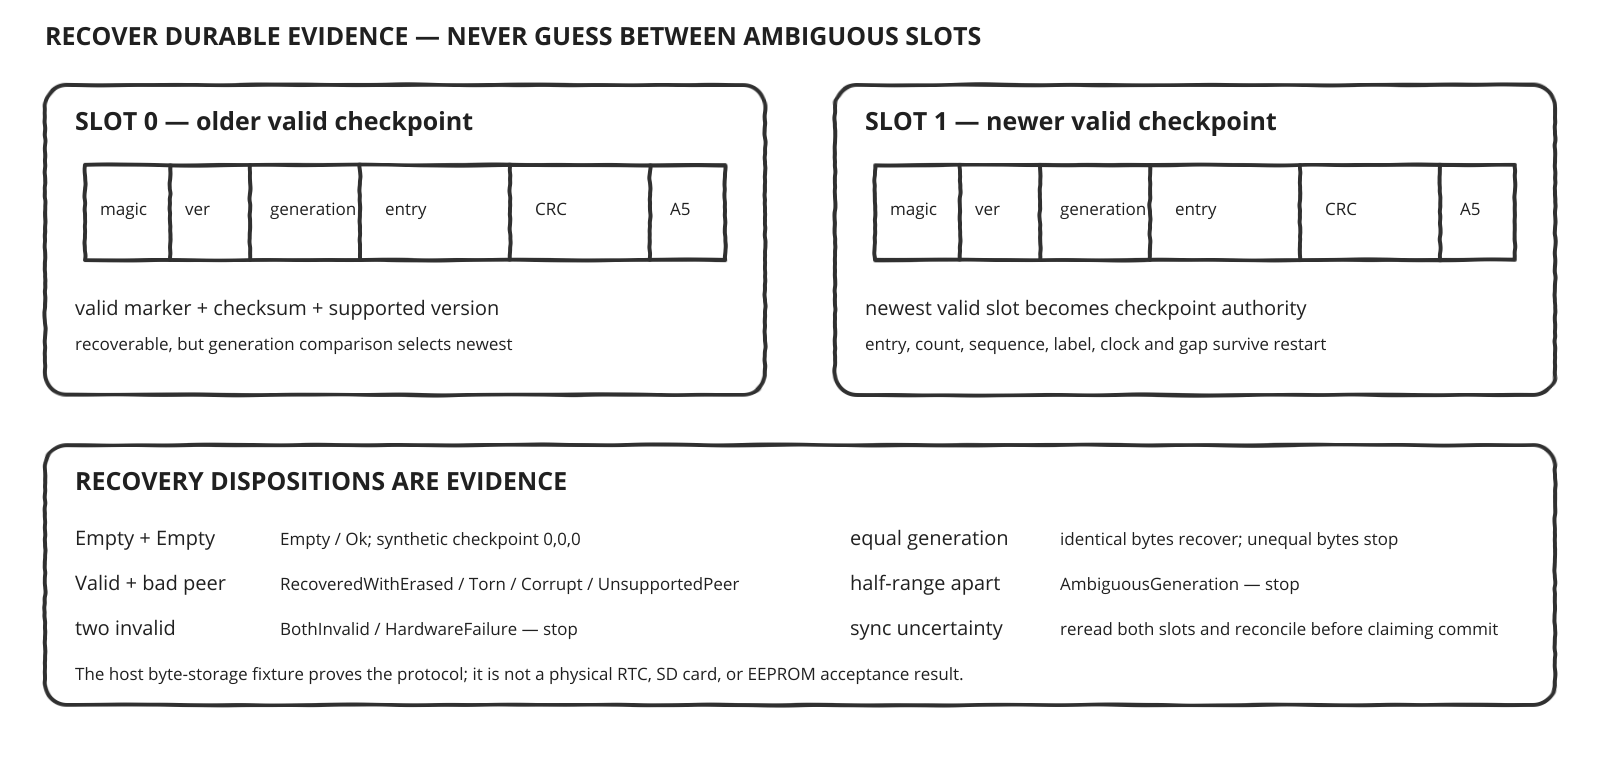
\includegraphics[width=0.98\linewidth]{036-ledger-recovery-pencil.png}

\small\textit{Alternative text: pencil drawings compare two alternating
fixed-size ledger slots; the newest supported valid slot wins, while erased,
torn, corrupt, duplicate-generation, unsupported-version, and ambiguous
generation states remain explicit recovery evidence.}
\end{center}

Each fixed-size slot stores magic, version, length, modular generation, the
fully encoded entry, resulting count and sequence, IEEE CRC-32, and valid
marker. Integer fields are explicitly little-endian; no C++ object memory
image is stored. Commit invalidates the inactive marker, writes body and
checksum in order, synchronizes, writes marker \texttt{0xa5} last, then
synchronizes again.

Two erased slots recover as Empty with synthetic checkpoint \(\{0,0,0\}\).
One valid supported slot wins over an erased, torn, corrupt, or unsupported
peer while preserving that disposition. Two invalid non-erased slots stop.
Equal generations recover only when bytes are identical. Unequal duplicate
generations and exact half-range separation are ambiguous and stop.

When synchronization fails, the ledger rereads both slots. It reports committed
after reconciliation only when the new checkpoint is provably newest; reports
not committed when the old checkpoint still wins; and becomes unusable when
the result or reread is ambiguous.

\section{Narrative example and evidence order}
\begin{lstlisting}[style=adkcpp]
void loop ()
{
    observeAcceptedPassage ();
    decideLabelAndCommit ();

    if (!actuateDurableEvidence ())
    {
        stopSafely ();
    }
}
\end{lstlisting}
The full fixture acquires indicator outputs and display, configures the
two-slot ledger, RTC fixture, and logger, then starts with recovered state
visible. Observe--decide--actuate order never makes presentation authoritative
over persistence.

\section{Predict, observe, interpret}
\begin{enumerate}
 \item Predict Empty recovery and displayed zero from two erased host slots.
 \item Submit one accepted record. Predict D30 and D31 together when clock,
       ledger, and presentation all succeed in the same call.
 \item Deliberately fail the RTC or ledger fixture. Predict D30 without D31,
       then retry the same sequence and observe D31 only after durable commit.
 \item Fail the first RTC read. Predict frozen pending input, no ledger write,
       then one new clock read on same-sequence retry.
 \item Fail a body write or synchronization. Predict no logical advance unless
       reread proves the new slot newest.
 \item Present a newer record while pending. Predict one overrun snapshot and
       no hidden queue.
 \item Corrupt the inactive peer and restart. Predict recovered durable entry
       plus explicit corrupt-peer disposition.
 \item In the host fixture, fail display presentation. Predict durable count
       unchanged and persistent fault. The canonical Mega sketch does not
       inject a display failure; it visibly demonstrates the RTC retry only.
\end{enumerate}

\section{Diagnosis and exercises}
\begin{tabularx}{\linewidth}{@{}X X@{}}
\toprule
Observation & Interpret and inspect\\
\midrule
D30 without D31 & accepted input is pending clock or ledger completion\\
D31 but display stale & durable commit succeeded; presentation failed\\
count changes before D31 & reject the fixture; presentation preceded authority\\
restart chooses older slot & inspect generation, marker, length, CRC, version\\
two slots disagree equally & stop; do not guess a winner\\
new input disappears & inspect bounded overrun evidence and caller policy\\
\bottomrule
\end{tabularx}
\begin{enumerate}
 \item Explain why the valid marker is written last.
 \item Trace an RTC failure followed by ledger failure and successful retry.
 \item Distinguish \texttt{RecoveredWithTornPeer} from \texttt{BothInvalid}.
 \item Explain why label and clock are excluded from equal-sequence comparison.
 \item Show why display failure cannot justify rewriting a ledger slot.
\end{enumerate}

\lessonbox{\textbf{Stop rule.} Use only deterministic RTC, byte-storage, and
accepted-passage fixtures plus the inert indicator panel. Remove USB for heat,
odor, reset, unstable rail, unexpected display/LED state, or current-limit
trip. Do not connect unknown sensors, physical RTC/media, motion, gates, locks,
vehicles, launchers, ignition paths, or safety systems.}

\section{Software evidence}
Host tests must cover directions and labels, recovery dispositions, every
byte/sync failure, byte-identical retry, torn restart, generation/sequence
edges, pending overrun, lifecycle rollback, display failure, and deterministic
trace/state bytes. Compilation, replay, this PDF, and host-slot recovery are
not physical persistence, RTC, sensor, or bench evidence. The searchable HTML
lesson is the primary accessible route. This PDF remains untagged and makes no
PDF/UA claim.

The Mega fixture deliberately fails its first abstract RTC read. D30 and D32
make the pending fault visible without D31; the same-sequence retry then
commits, and a bounded two-second persistent-fault interval ends with
shutdown/reinitialization and recovery from the retained software slots.
The D28 pull-up button cycles \texttt{None/A/B/C}; its edge is applied after
the current logger update, so a simultaneous press affects only the next new
sequence. Its bounded one-second \texttt{-/A/b/C} preview then restores the
durable count.

\section{What the result establishes}

A passing fixture establishes deterministic policy: accepted data freezes
before clock and ledger work; retries preserve the right bytes; a durable
checkpoint precedes presentation; recovery never silently chooses ambiguous
evidence; and bounded overrun remains visible. It does not establish EEPROM or
SD wear life, RTC accuracy, power-loss behavior on a physical board, sensor
identity, passage geometry, current margin, or suitability for access control.

\begin{tabularx}{\linewidth}{@{}l X@{}}
\toprule
Authority & Consult it for\\
\midrule
\texttt{magnetic\_passage\_logger.h} & lifecycle, pending, pulse, and status contract\\
\texttt{passage\_ledger.h} & slot recovery and commit interface\\
focused host tests & failure, retry, recovery, and deterministic byte evidence\\
Lessons 034--036 design record & frozen policy and deferred physical gates\\
testing and safety contracts & evidence language, current limits, and stop rules\\
\bottomrule
\end{tabularx}

The HTML lesson remains the searchable companion. Exact physical components
need primary sources, an authoritative schematic, current accounting, and a
recorded human bench result before any support or persistence claim.
\end{document}
